\chapter{Asking Yacht Owners How They Got RICH!}

This chapter has no blackboard in the ordinary sense, but it does have a quantitative spine. We begin with visible wealth, then we keep asking what structure lies underneath it: what kind of business throws off enough cash to support a yacht, what separates seven figures from eight, why raw earnings are not yet the same thing as durable wealth, and what hidden supports make confidence and scale possible. The lecture proceeds interview by interview, and we will keep that order, letting each answer sharpen the previous one rather than replacing it.

\section{Wealth on the Water}

The lecture opens with a simple field-theoretic observation: a yacht appears, and the host refuses to leave it at the level of image. The boat is treated as data. What matters is not merely that it is there, but that it must have been paid for, maintained, staffed, and folded into some larger economic machine.

The host then broadens the frame from one encounter to a whole city. Miami is presented as a natural laboratory for the question because visible luxury is unusually concentrated there, and because the city provides repeated contact with the class of people whose commercial logic the lecture wants to extract.

\begin{equation}
N_{\text{Miami millionaires}} \approx 4.0\times 10^{4}.
\end{equation}

This number is not used analytically in the lecture, but it does set the scale of the problem. We are not dealing with a freak case. We are dealing with an environment in which the visible signs of wealth appear often enough to invite pattern recognition.

From there the lecture makes its first move: we stop speaking about millionaires in the abstract, and we walk toward the first marina.

\section{First Marina: Numbers Before Philosophy}

The first full interview gives the chapter its cleanest numerical anchor. The subject is in e-commerce, has been operating for about four years, is $22$ years old, says he became a millionaire at $19$, and reports a very large recent year.

\begin{align}
R &\approx \$32\,\mathrm{M}, &
P &\approx \$19\,\mathrm{M}, &
a &= 22, &
t_{\text{millionaire}} &= 19.
\end{align}

Here \(R\) denotes annual revenue, \(P\) denotes annual profit, \(a\) is the current age, and \(t_{\text{millionaire}}\) is the age at which millionaire status was reached. The lecture does not present these as a formal model, but it does present them as the first serious answer to the opening question.

\paragraph{Worked Example.}
A useful derived quantity is the implied margin:
\begin{equation}
m := \frac{P}{R} \approx \frac{19}{32} \approx 0.59.
\end{equation}

So on the fuller version of the first interview, and only on that fuller version, we obtain an implied profit margin of roughly \(59\%\). We should immediately note that the cold open contains montage-like fragments --- \(\$25\) million, \(\$30\) million, \(\$19\) million in profit, \(\$10\) million --- and those fragments should not be merged into a single clean dataset. The calculation above uses the more coherent interview passage.

The lecture does not stay with the money for long. Almost at once it turns from output to biography: maternal death in childhood, violence in adolescence, expulsion from college, and millionaire status at nineteen. The point is not merely inspirational. The interviewee is trying to say that adversity did not interrupt the path; adversity became part of the internal mechanism that later handled scale.

\subsection{Question \& Answer}

\paragraph{Question.}
How do we move from seven figures to eight?

\paragraph{Answer.}
The answer begins by denying that the old mode of operation can simply be extended. According to the lecture, seven figures may be reachable while one is still operating in a largely solo mode; eight figures requires a change in structure. The founder must stop trying to be the entire machine.

This is the first real commercial theorem of the chapter. The lecture introduces it here because the numerical claims have created enough tension that a mere autobiographical answer would be insufficient. We now need a mechanism.

\section{Delegation and the Founder-Time Bottleneck}

The core scaling claim of the first interview is that time, not talent in the abstract, becomes the bottleneck.

\begin{equation}
A_{\text{founder}} = T_f,
\end{equation}
where \(A_{\text{founder}}\) is the founder's most valuable scarce asset and \(T_f\) is founder time.

The lecture's verbal logic can be compressed into the following schematic:
\begin{equation}
S_7 \to S_8 \Rightarrow \text{delegate work} + \text{release founder time}.
\end{equation}

Here \(S_7\) and \(S_8\) are only editorial shorthand for seven-figure and eight-figure operating regimes. The lecture itself is not introducing a symbolic formalism. But the underlying point is sharp enough that some notation is useful.

A second compression is equally important:
\begin{equation}
I_f \to L_w \to O,
\end{equation}
where founder ideas \(I_f\) are handed off to worker labor \(L_w\), producing output \(O\). The interviewee's language is blunt: the entrepreneur should create ideas and delegate them; workers then execute for a fraction of the value captured at the top of the structure.

\begin{figure}[h]
\centering
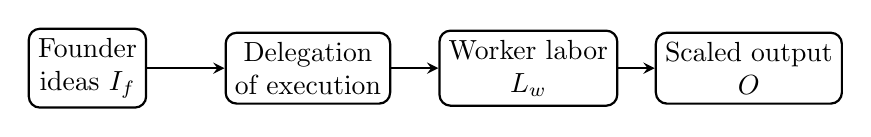
\begin{tikzpicture}[>=stealth, thick, node distance=2.8cm]
\node[draw, rounded corners, align=center] (ideas) {Founder\\ideas \(I_f\)};
\node[draw, rounded corners, right of=ideas, align=center] (delegate) {Delegation\\of execution};
\node[draw, rounded corners, right of=delegate, align=center] (workers) {Worker labor\\\(L_w\)};
\node[draw, rounded corners, right of=workers, align=center] (output) {Scaled output\\\(O\)};
\draw[->] (ideas) -- (delegate);
\draw[->] (delegate) -- (workers);
\draw[->] (workers) -- (output);
\end{tikzpicture}
\end{figure}

This diagram is not recovered from a board; it is a clean summary of the lecture's verbal structure. It sits close to the transcript because the interviewee keeps repeating the same distinction in different idioms: free thinker and worker, idea and execution, founder and educated hire, bottleneck and release.

The lecture then adds a second layer. Delegation alone is not enough; one must also hire upward. The speaker stresses that he is not the smartest person in the room and names employees with Yale, Stanford, and Harvard backgrounds. The argument is not anti-education in any simple sense. It is instead a claim that the founder's job is to assemble intelligence, not to impersonate it all personally.

The most compressed heuristic in this part of the lecture is the mindset claim:
\begin{equation}
\text{Success bottleneck} \sim 0.8\,M + 0.2\,K,
\end{equation}
where \(M\) is mindset and \(K\) is skill set.

This should be read as a speaker's rule of thumb, not as a measured decomposition. Still, it explains the next verbal move. The lecture says that if we handed a million dollars to most people, they would be broke again in six months, not because they are stupid, but because they do not know how to steward and multiply capital. In that language, mindset is not optimism alone; it is custody.

The host then performs an important recap. He restates the lesson in simpler language: the number one thing keeping people broke is mindset. This is the lecture's way of freezing the first interview into a portable result before we move to a new location and a new voice.

\section{Older Wealth and the Question of What Counts}

The second substantial interview changes tempo. We move from a fast, young scaling story to an older owner who has moved through multiple industries: clubs, jewelry, gambling, film, and more. Instead of pressing further into operational leverage, the lecture now asks what wealth means once one has seen enough of it.

The answer comes through paired comparisons. Rick gives a paraphrased saying attributed to Steve Jobs: a Timex and a Rolex both tell the time, and a Volkswagen and a Rolls Royce both get you where you are going.

\begin{align}
\text{Timekeeping}(\text{Timex}) &= \text{Timekeeping}(\text{Rolex}),\\
\text{Transport}_{A\to B}(\text{Volkswagen}) &= \text{Transport}_{A\to B}(\text{Rolls Royce}).
\end{align}

These are obviously not equations of price, symbolism, or social effect. They are equations of core function. The lecture uses them to cut against the temptation created by the opening spectacle. If we begin with a yacht, we may too easily confuse visible luxury with the thing that matters. This interview insists that utility and status are different variables.

\subsection{Question \& Answer}

\paragraph{Question.}
If money buys status, what actually matters?

\paragraph{Answer.}
Rick answers by displacing the whole coordinate system. It is not finally a question of money. It is a question of how one treats life, oneself, and others; it is a question of what one learns after bottom; it is a question of self-knowledge. The lecture uses this answer to slow us down. The yacht is still there, but it no longer monopolizes the meaning of success.

This same interview also complicates the educational theme. He says that if he had more education he might have gone further earlier, but he does not equate a college degree with success. Education, in this frame, improves decisions; it does not mechanically guarantee reward.

The next pivot follows naturally. Once education has been made contingent rather than absolute, the lecture asks again for the common denominator across successful people.

\section{Risk, Education, and the Unteachable Element}

The third interview provides that denominator in a sharper form. Education may help one make better decisions, but risk remains indispensable.

\begin{equation}
\text{no risk} \Rightarrow \text{no reward}.
\end{equation}

That is the compact commercial law of this section. But the lecture does not stop there. Risk-taking by itself is still not the deepest term. When the host asks how self-belief was found, Franco says something harsher: belief cannot be taught. One either enters the game with it, cultivates it internally, or does not enter at all.

\subsection{Question \& Answer}

\paragraph{Question.}
Can self-belief be taught?

\paragraph{Answer.}
The lecture's answer here is largely no. Skills may be transferred, degrees may provide tools, but the decisive willingness to believe in oneself and make the leap is treated as irreducible. The host's own summary reinforces this: what distinguished the speaker was not a single taught skill nor an external benefactor, but an unwavering belief that success would be achieved.

This section works structurally because it reopens the problem from the opposite direction. The first interview gave us mechanics; the second gave us proportion; the third gives us the condition under which any of the mechanics are even entered into.

\section{Hunger, Pillars, and Confidence as Process}

The final substantive interview gathers the scattered pieces and folds them into a thicker support model. The question about what all highly successful people share is answered first with hunger and execution. They are not merely imaginative; they are hungry enough to act on their own schemes.

Then the lecture turns again. Hunger is not presented as self-sufficient. The speaker names scripture, faith, wife, long-term friends, and a circle of spiritual supports. When the path turns rocky, the real question is: what does one hang on to?

We can represent the named support structure schematically as
\begin{equation}
\mathcal{P}=\{\text{faith},\ \text{marriage},\ \text{long-term friends}\}.
\end{equation}

This is not the lecture's notation, only a compact way of recording the list. The point is that endurance is supported, not solitary.

\subsection{Question \& Answer}

\paragraph{Question.}
What do we hang on to when scaling gets rocky?

\paragraph{Answer.}
The lecture's answer is not an abstract doctrine. It is a support structure: faith, spouse, and the friends who have been there for years. One may say that confidence is internal, but this interview insists that internal steadiness is held up by external and spiritual pillars.

The chapter ends with the closest thing it has to a genuine update rule. The speaker tells the audience that confidence is not wished into being. It is built by keeping promises to oneself, one day at a time. In a compressed form we may write
\begin{equation}
G_d \to C \to G_{\text{larger}},
\end{equation}
where repeated daily goal completion \(G_d\) produces confidence \(C\), and that confidence permits pursuit of larger goals \(G_{\text{larger}}\).

The verbal derivation is explicit enough to record step by step:
\begin{enumerate}
\item We make daily promises to ourselves.
\item We keep those promises.
\item Kept promises accumulate into completed daily goals.
\item Completed daily goals accumulate into confidence.
\item Confidence allows us to attempt and hold larger goals.
\end{enumerate}

This closing move is important because it prevents the lecture from collapsing into pure charisma. Confidence, in this final account, is not a mysterious aura; it is the visible residue of repeated fulfilled commitments.

\section{Summary}

The lecture begins by treating a yacht as a question mark and ends by dissolving the yacht into a deeper structure. First come the numbers: revenue, profit, age, and speed. Then comes the first mechanism: the shift from solo effort to delegation, and the recognition that founder time is the scarce asset. After that the chapter broadens: function matters more than display, education may sharpen judgment without being destiny, risk and self-belief remain decisive, and durable confidence rests on discipline and support rather than on spectacle alone.

So the lecture's commercial mathematics is simple but not thin. We begin with visible wealth, write down the strongest numbers we can trust, derive a few ratios, and then keep following the hidden variables: time, leverage, stewardship, risk, pillars, and confidence. That is the real object underneath the boat.